 \section{Introduction}
 
\lipsum[5-7] Image shows an image.

 \renewcommand{\baselinestretch}{1.5}
\begin{figure}[!htbp]
	\centering
	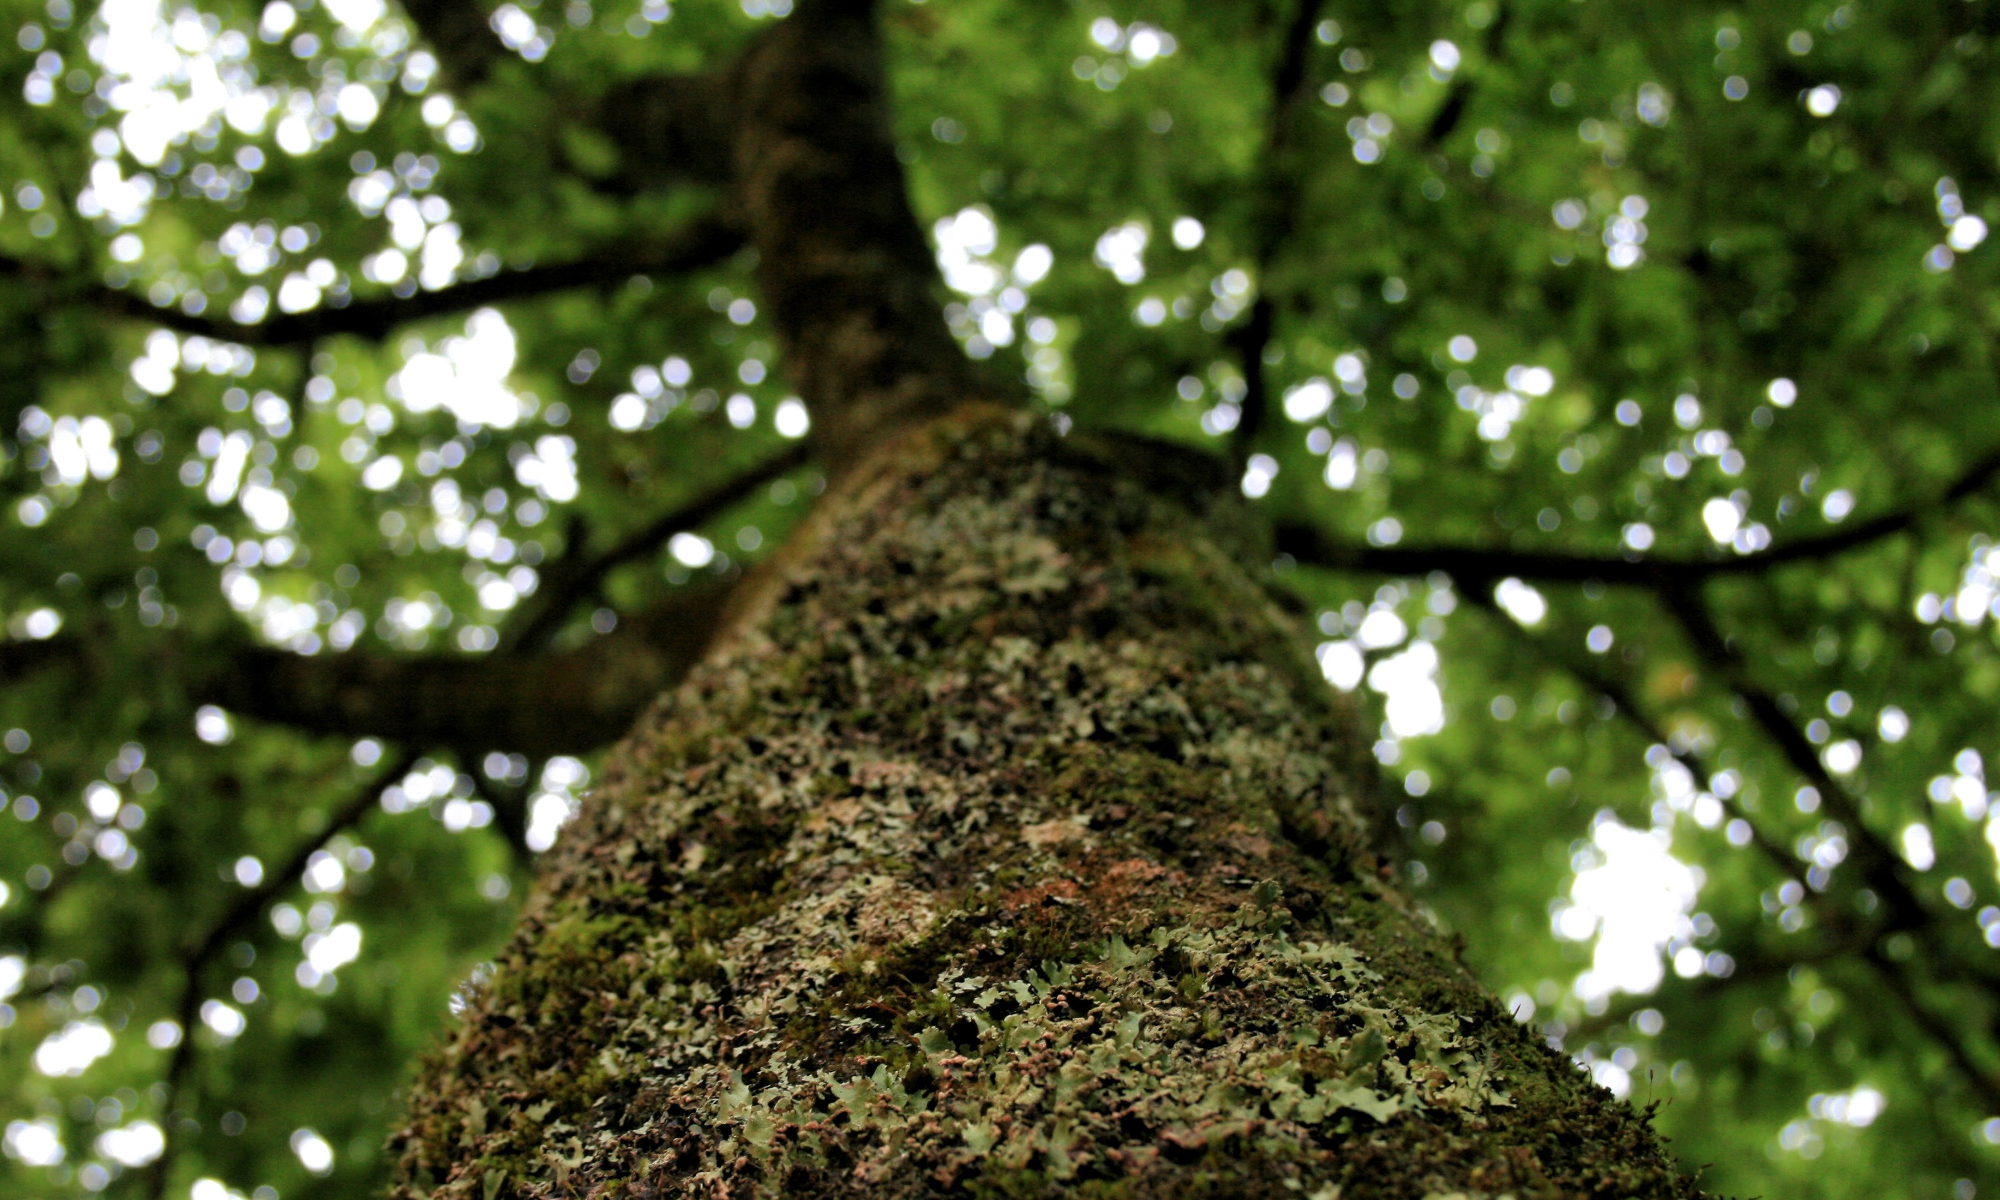
\includegraphics[width=\textwidth]{chapter1figure1}
	\caption[This title will appear in the TOC]{This is a longer more descriptive image caption.}
	\label{fig:chapter1figure1}		
\end{figure}
\renewcommand{\baselinestretch}{2.0}

\lipsum[7-8]
 
 
\section{Next Section}
 
\lipsum[9-10] Equation \ref{eqn:force} shows the fundamental relationship between force, mass, and acceleration. 

 	\begin{equation}
	F = m\times a
	\label{eqn:force}
	\end{equation}
	
\lipsum[11]

\subsection{Sub-Section}

\lipsum[1]. Table \ref{chapter1table1} is an example of a horizontal table on a landscape page.

\renewcommand{\baselinestretch}{1.5}
\begin{landscape}
	\begin{table}[p]
 		\centering
		\caption{This Is A Table}
		\label{chapter1table1}
		\resizebox{.8\textwidth}{!}{% based on the table you can change the multiplier for text width to fill as much or as little of the page as you want
\begin{tabular}{@{}ccccc@{}}
	\toprule
	\textbf{Section 1} & \textbf{Section 2} & \textbf{Section 3} & \textbf{Section 4} & \textbf{Section 5} \\ \midrule
	\textbf{1}         & Red                & Blue               & Green              & Yellow             \\
	\textbf{2}         & Orange             & Red                & Blue               & Green              \\
	\textbf{3}         & Yellow             & Orange             & Red                & Blue               \\
	\textbf{4}         & Green              & Yellow             & Orange             & Red                \\
	\textbf{5}         & Blue               & Green              & Yellow             & Orange             \\
	\textbf{6}         & Red                & Blue               & Green              & Yellow             \\
	\textbf{7}         & Orange             & Red                & Blue               & Green              \\
	\textbf{8}         & Yellow             & Orange             & Red                & Blue               \\
	\textbf{9}         & Green              & Yellow             & Orange             & Red                \\ \bottomrule
\end{tabular}%
}
	\begin{center}
	\small This is the caption of the table.
	\end{center}
\end{table}
\end{landscape}
\renewcommand{\baselinestretch}{2}
 
The following is a list:
\begin{enumerate}[label=\textbf{(\arabic*)}]
 	\item This
 		\item Is
 			\item A
 				\item List
  \end{enumerate}
 
 
 
 
 